\documentclass[a4paper,11pt]{scrartcl}
\usepackage[T1]{fontenc}
\usepackage[utf8]{inputenc}
\usepackage{lmodern}
\usepackage[spanish]{babel}
\usepackage{mathtools}
\usepackage{amssymb, amsmath, amsbsy}
\usepackage{enumerate}
\usepackage{graphicx}
\usepackage{subfigure}
\usepackage{hyperref}

\title{Cinemática de la partícula}
\subtitle{Primer Examen Parcial \\ Equipo 12}
\author{
  Aguilar Enriquez Paul Sebastian\\
  \and
  Benitez Barroso Brandon Raul\\
  \and
  Castillo Herrera Gabriela\\
  \and
  Martinez Vidal Joceline Yadira\\
  \and
  Milán Hernández Maria Fernanda
  }
\date{29 de agosto del 2016}
\begin{document}

\maketitle

\begin{center}
  Repositorio del documento en GitHub
  \url{https://github.com/penserbjorne/clase-cinematicaydinamica-2017-1}
\end{center}

\textbf{Ejercicio 1} El movimiento de una partícula en una dimensión está dada por la ecuación $x(t)= \alpha t^{2} + \beta + \gamma cos(\omega t)$ donde $t$ representa al tiempo. Determina las expresiones para la velocidad $v$ y aceleración $a$ como funciones del tiempo. Si $\alpha = 6 \frac{m}{s^{2}}$, $\beta = -8 m$, $\gamma = 40 m$ y $\omega = \pi \frac{rad}{seg}$. Determina los vlores de $v(t)$ y $a(t)$ cuando $t = 6 s$.\\

\textbf{Solución:}

\begin{center}

Primero se deriva {\bf x(t)} para así obtener la {\bf v(t)} \\

\begin{equation}
v(t) = \frac{d x(t)}{dt}  = 2\alpha t - \gamma \omega sen(\omega t)
\end{equation}

Después se deriva {\bf v(t)} para poder obtener la {\bf a(t)} \\

\begin{equation}
a(t) = \frac{d v(t)}{dt} = 2\alpha - \gamma \omega^{2}cos(\omega t)
\end{equation}

Por útimo sustituimos los valores dados del problema:

\hfill \break

$\alpha = 6 [\frac{m}{s^{2}}], \beta = -8 [m], \gamma = 40 [m], \omega = \pi [\frac{rad}{s}]$ y $t = 6 [s]$

\hfill \break

\hfill \break

En {\bf v(t)}:\\

\begin{equation}
v(6[s]) = 2(6[\frac{m}{s^{2}}])(6[s]) - (40[m])(\pi [\frac{rad}{s}])sen(((\pi [\frac{rad}{s}])(6[s]))
\end{equation}

\begin{equation}
v(6[s]) = 72[\frac{m}{s}] - (40[m])(\pi [ \frac{rad}{s}])(0)
\end{equation}

\begin{equation}
v(6[s]) = 72[\frac{m}{s}]
\end{equation}

En {\bf a(t)}:\\

\begin{equation}
a(6[s]) = 2(6[\frac{m}{s^{2}}]) - (40[m])(\pi [\frac{rad}{s}])cos(((\pi [\frac{rad}{s}])(6[s]))
\end{equation}

\begin{equation}
a(6[s]) = 12([\frac{m}{s^{2}}]) - 394.78 [\frac{m}{seg^{2}}]
\end{equation}

\begin{equation}
a(6[s]) = - 394.78 [\frac{m}{s^{2}}]
\end{equation}

Por lo tanto tenemos que la velocidad y la aceleracion en el tiempo $t = 6s$ es:\\

\begin{equation}
  \left\lbrace
  \begin{array}{l}
     v(6[s]) = 72[ \frac{m}{s}]\\
     a(6[s]) = - 394.78 [ \frac{m}{s^{2}}]\\
  \end{array}
  \right.
\end{equation}

\end{center}

\textbf{Ejercicio 3} La aceleración de un objeto que se mueve en una dimensión está dada por $a( x(t) ) = - \omega^{2}x(t)$, donde $\omega > 0$ es una constante con unidades $\frac{rad}{s}$. (a) Muestra  que  la expresión para la posición como función de tiempo es de la forma $x(t) = A sen ( \omega t ) + B cos ( \omega t )$. (b) Si definimos $\widetilde{T} = \frac{1}{2}(v^{2}-v_0^{2})$ y $\widetilde{V} = -\frac{\omega^{2}}{2}(x^{2}-x_0^{2})$, muestra que entonces $\widetilde{T} = \widetilde{V}$ para todo tiempo t.\\

\textbf{Solución:}

\begin{center}

(a) Garantizando que es la solución:\\

\begin{equation}
x(t) = A sen ( \omega t ) + B cos ( \omega t )
\end{equation}

Derivamos\\

\begin{equation}
\frac{dx}{dt} = A \omega cos ( \omega t ) - B \omega sen ( \omega t )
\end{equation}

Volvemos a derivar\\

\begin{equation}
\frac{d^{2}x}{dt^{2}} = - A \omega^{2} sen ( \omega t ) - B \omega^{2} cos ( \omega t )
\end{equation}

Factorizando\\

\begin{equation}
\frac{d^{2}x}{dt^{2}} = - \omega^{2} (\underbrace{A sen ( \omega t ) - B cos ( \omega t )}_{{x(t)}}) = - \omega^{2}x(t)
\end{equation}

$\therefore$ la expresión para la posición como función de tiempo es de la forma $x(t) = A sen ( \omega t ) + B cos ( \omega t )$\\

\hfill \break

(b) De otra forma\\

\hfill \break

$a(x) = v\frac{dv}{dx}$ en lugar de $a(x) = \frac{dv}{dt}$ ya que la segunda depende del tiempo\\

\begin{equation}
a(x) = v\frac{dv}{dx} = - \omega^{2}x
\end{equation}

Separamos variables y definimos integrales\\

\begin{equation}
\int_{v_0}^{v} v' dv' = - \omega^{2} \int_{x_0}^{x} x' dx'
\end{equation}

Integrando\\

\begin{equation}
\frac{v^{2}-v_0{2}}{2} = - \omega^{2} \frac{x^{2}-x_0{2}}{2}
\end{equation}

\begin{equation}
\frac{1}{2}(v^{2}-v_0{2}) = - \frac{\omega^{2}}{2}(x^{2}-x_0{2})
\end{equation}

\begin{equation}
\therefore \widetilde{T} = \widetilde{V}
\end{equation}
 
\end{center}

\textbf{Ejercicio 11} Después de despegar, un helicóptero vuela en línea recta haciendo un ángulo $\beta$ con respecto al suelo. Simultáneamente, un radar sigue su movimiento en el punto A como se observa en la figura~\ref{fig:11_1}. Determina la velocidad del helicóptero en términos de $d, \beta, \theta$ y $\dot{\theta}$.\\

\begin{figure}[h!]
  \centering
  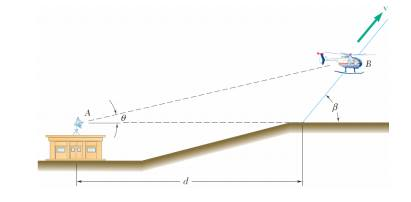
\includegraphics[width=0.7\textwidth]{11_1}
  \caption{Helicóptero despegando en el Problema 11.}
  \label{fig:11_1}
\end{figure}

\textbf{Solución:}

\begin{center}

De acuerdo a la geometría (figura~\ref{fig:11_2}) \\

\begin{figure}[h!]
  \centering
  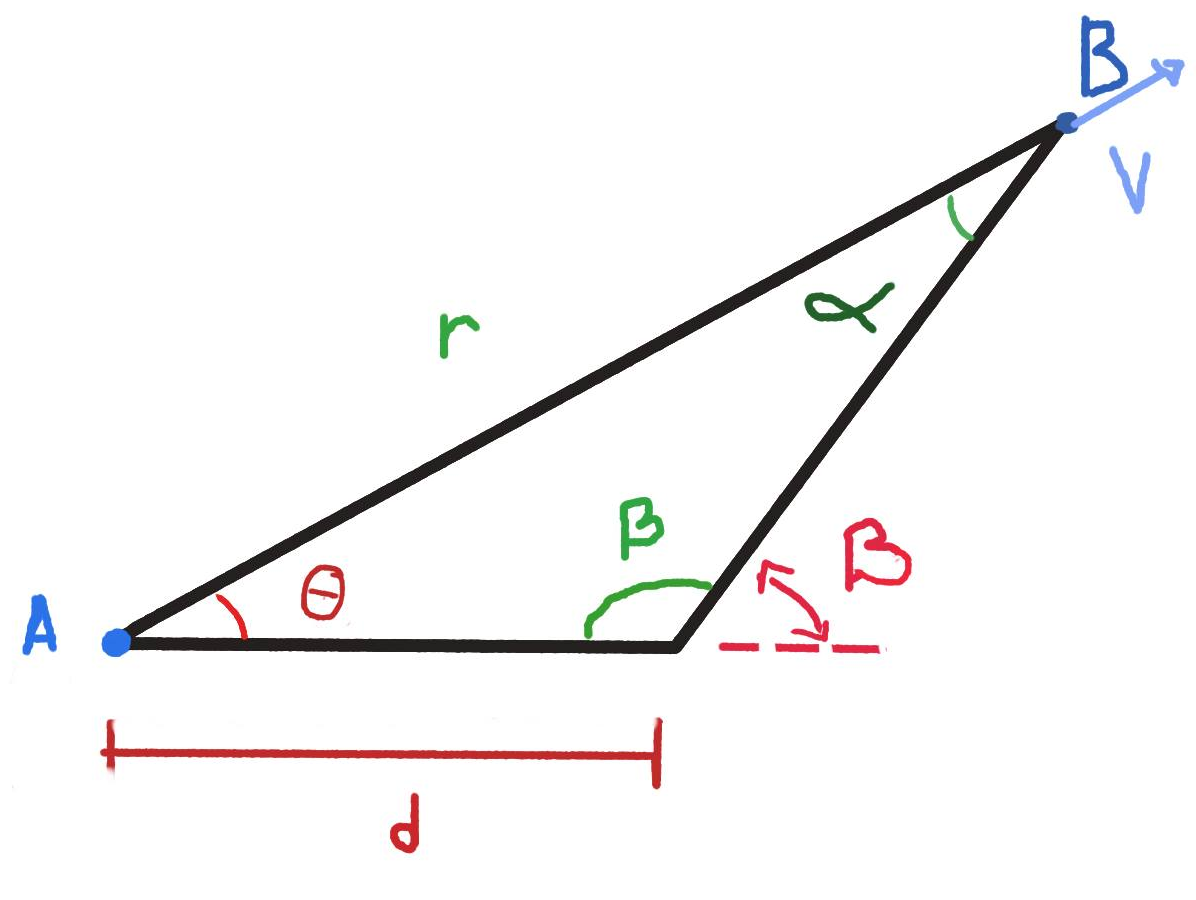
\includegraphics[height=4cm]{11_2}
  \caption{Geometria del planteamiento del problema}
  \label{fig:11_2}
\end{figure}

\begin{equation}
\theta + (180^{\circ} + \beta) + \alpha = 180^{\circ}
\end{equation}

\begin{equation}
\alpha = 180^{\circ} - (180^{\circ} - \beta) - \theta
\end{equation}

\begin{equation}
\alpha = \beta - \theta
\end{equation}

\begin{figure}[h!]
  \centering
  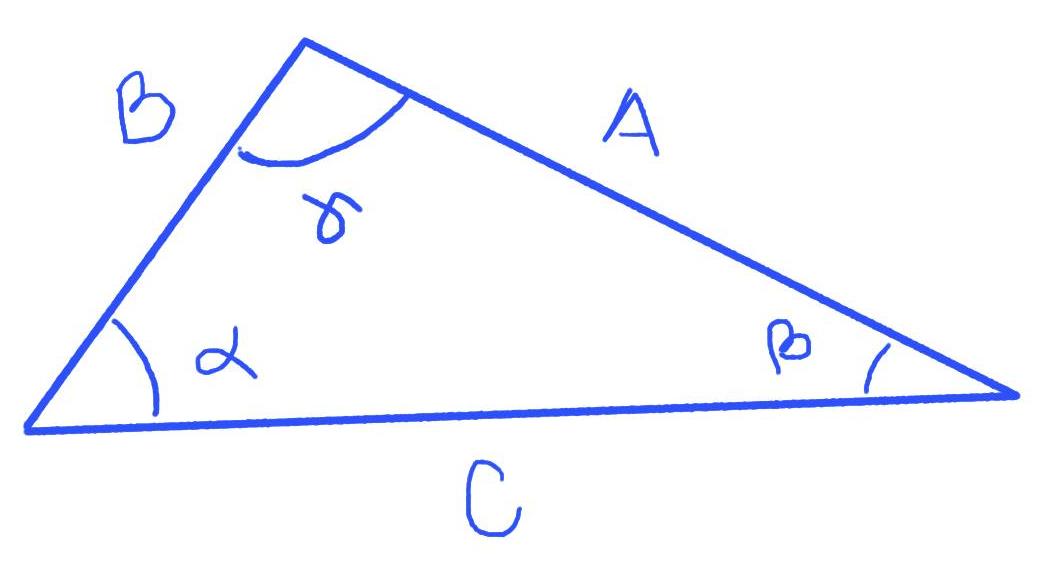
\includegraphics[height=3cm]{11_3}
  \caption{Triangulo para representar la ley de senos y cosenos}
  \label{fig:11_3}
\end{figure}

Respecto a la ley de los senos (figura~\ref{fig:11_3})\\
\hfill \break
$\frac{A}{sen(\alpha)}$ = $\frac{B}{sen(\beta)}$ = $\frac{C}{sen(\gamma)}$\\
\hfill \break
Entonces tenemos:\\

\begin{equation}
\frac{r}{sen(180^{\circ} - \beta)} =  \frac{d}{sen(\alpha)}
\end{equation}

\begin{equation}
\frac{r}{sen(180^{\circ} - \beta)} = \frac{d}{sen(\beta - \theta)}
\end{equation}

Recordando que:\\
\hfill \break
$sen(\alpha - \beta) = sen(A)cos(B) - cos(A)se(B)$\\
\hfill \break
Podemos realizar lo siguiente:\\

\begin{equation}
r sen(\beta - \theta) = d (sen(180^{\circ} - \beta))
\end{equation}

\begin{equation}
r sen(\beta - \theta) = d (sen(180^{\circ})cos(\beta) - cos(180^{\circ})sen(\beta))
\end{equation}

\begin{equation}
r sen(\beta - \theta) = d (sen(\beta))
\end{equation}

\begin{equation}
r sen(\alpha) = d (sen(\beta))
\end{equation}

\begin{equation}
r = \frac{d(sen(\beta))}{sen(\alpha)}
\end{equation}

\begin{figure}[htbp]
\centering
\subfigure[]{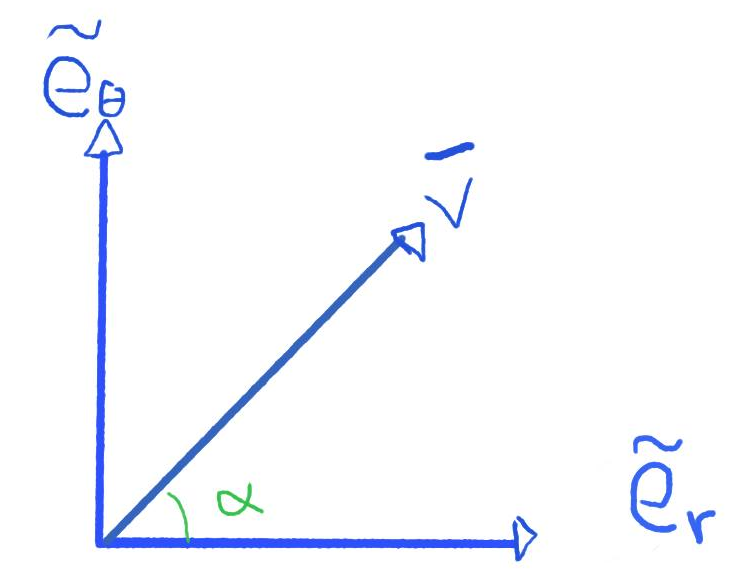
\includegraphics[height=4cm]{11_4}}
\subfigure[]{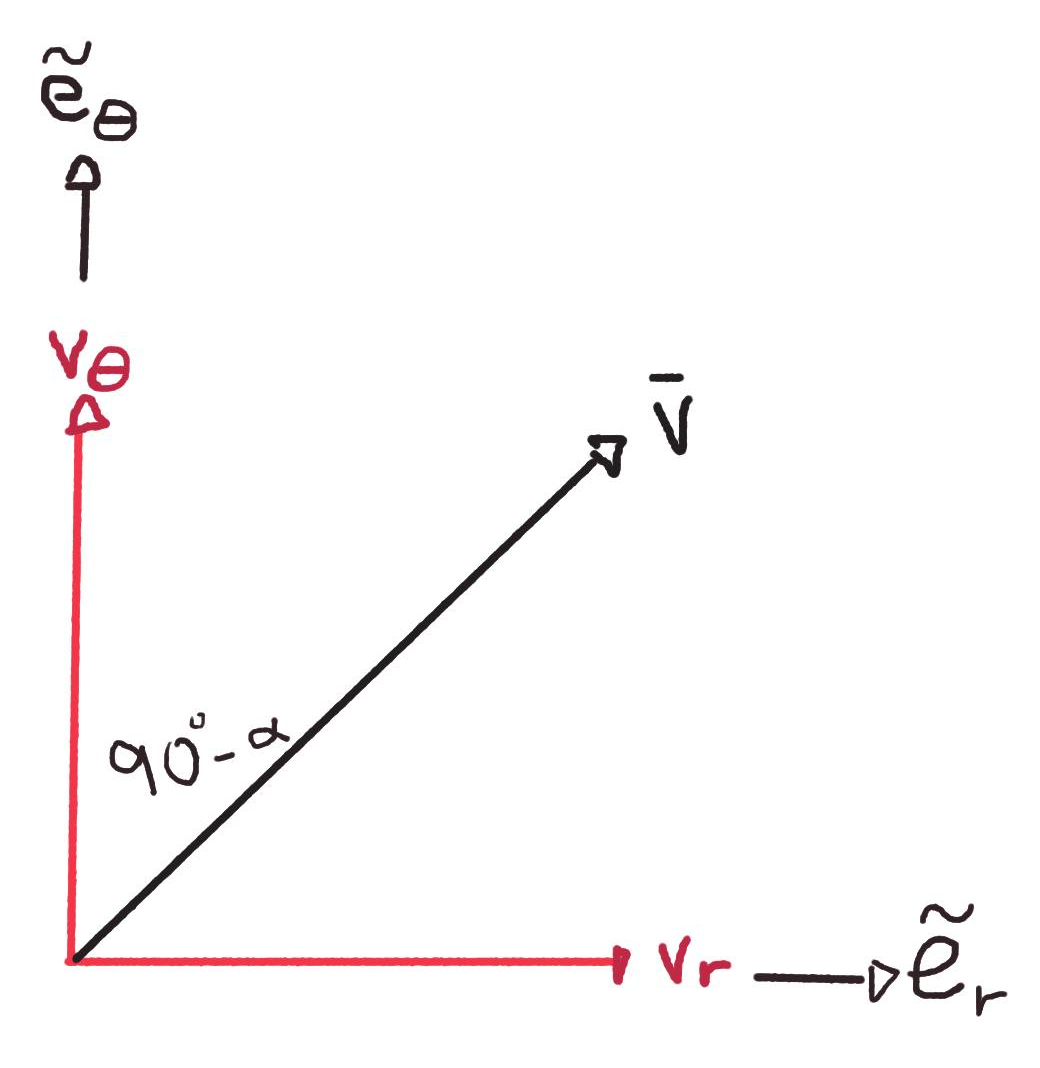
\includegraphics[height=4cm]{11_5}}
\subfigure[]{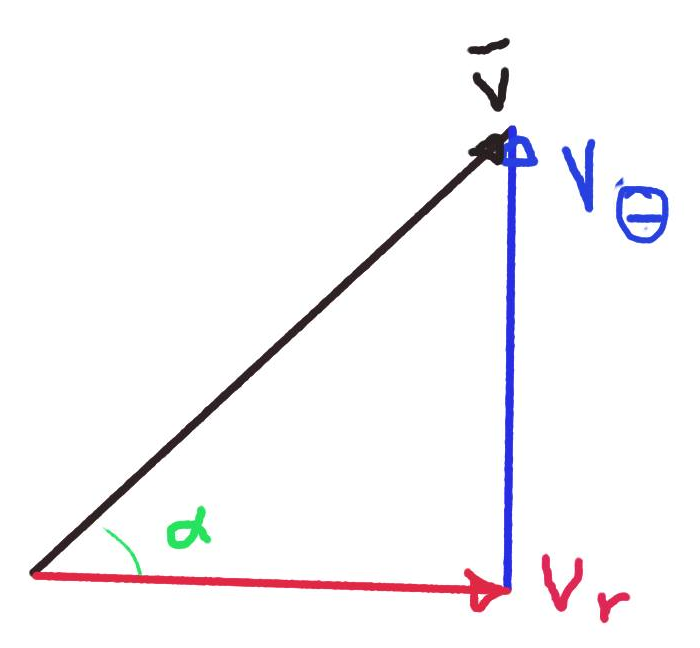
\includegraphics[height=4cm]{11_6}}
\caption{Vector Velocidad}
\label{fig:vector_velocidad}
\end{figure}

A partir del dibujo del vector velocidad (figuras ~\ref{fig:vector_velocidad}):\\

\begin{equation}
v_{\theta} = v cos(90^{\circ} - \alpha) = v \hat{e_{\theta}}
\end{equation}

\begin{equation}
v_{\theta} = v sen(\alpha)
\end{equation}

Como se demostró en clase, sabemos que:\\
\hfill \break
$v_{\theta} = r \dot{\theta}$\\
\hfill \break
Sustituyendo por las variables conocidas:\\

\begin{equation}
v_{\theta} = r \dot{\theta}
\end{equation}

\begin{equation}
v sen(\alpha) = (\frac{d sen(\beta)}{sen(\alpha)}) \dot{\theta}
\end{equation}

\begin{equation}
v = \frac{\frac{d sen(\beta)}{sen(\alpha)} \dot{\theta}}{\frac{sen(\alpha)}{1}}
\end{equation}

$\therefore$ el resultado es:\\

\begin{equation}
  \left\lbrace
  \begin{array}{l}
v = \frac{d sen(\beta)}{sen^{2}(\alpha)} \dot{\theta} = \frac{d sen(\beta)}{sen^{2}(\beta - \theta)} \dot{\theta}
  \end{array}
  \right.
\end{equation}
\end{center}

\textbf{Ejercicio 12} Un avión es detectado por un radar exactamente en la parte más baja de un \textit{loop}, como se
muestra en la figura~\ref{fig:12_1}. Si el aeroplano cambia su velocidad a una razón $a_t$ conocida, y el radio de curvatura en ese instante es $\rho$ , ¿cuáles son los valores de $\dot{r}$, $\ddot{r}$, $\dot{\theta}$ y $\ddot{\theta}$ detectados por el radar en ese instante? Evalúa las expresiones obtenidas para cuando $\rho = 2000 m$, $v_0 = 150 \frac{m}{s}$, $a = 800 m$, $b = 600 m$ y $a_t = 25 \frac{m}{s^{2}}$.\\

\begin{figure}[h!]
  \centering
  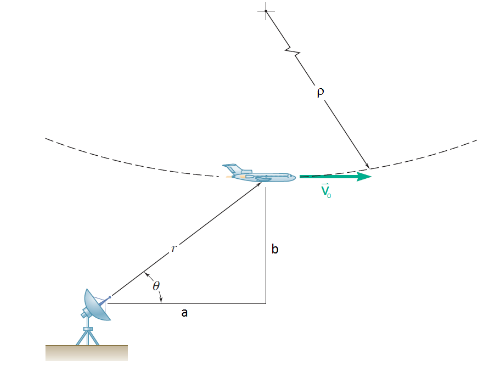
\includegraphics[width=0.7\textwidth]{12_1}
  \caption{Momento de la detección del aeroplano del Problema 12.}
  \label{fig:12_1}
\end{figure}

\textbf{Solución:}

\begin{center}

\begin{equation}
\bar{r} = r\hat{r}
\end{equation}

\begin{equation}
\bar{v} = \frac{d\bar{r}}{dt} = \dot{r}\hat{r} + r\dot{\hat{r}} = \dot{r}\hat{r} + r\dot{\theta}\hat{r}
\end{equation}

Sabemos que $\hat{x} = cos(\theta)\hat{r} - sen(\theta)\hat{\theta} \therefore$\\

\begin{equation}
\bar{v} = v_r\hat{r} + v_\theta\hat{\theta} = v_0\hat{x} = v_0 cos(\theta)\hat{r} - v_0 sen(\theta)
\end{equation}

Sabemos que $\dot{\hat{r} = \dot{\theta}\hat{\theta}}$  y $\dot{\hat{\theta}} = \dot{\theta}\hat{\theta} \therefore$\\

\begin{equation}
  \bar{v} = v_0 cos(\theta)\hat{r} - v_0 sen(\theta) = \dot{r}\hat{r} + r\dot{\theta}\hat{\theta}
\end{equation}

Igualando termino a termino\\

\begin{equation}
  v_0 cos(\theta) = \dot{r} \to \dot{r} = v_0 cos(\theta)
\end{equation}

\begin{equation}
  -v_0 sen(\theta) = r\dot{\theta} \to \dot{\theta} = -\frac{v_0 sen(\theta)}{r}
\end{equation}

Sustituyendo los valores numericos en $\dot{r}$ y $\dot{\theta}$\\

\begin{equation}
  \left\lbrace
  \begin{array}{l}
  \dot{r} = (150 \frac{m}{s})(\frac{800 m}{\sqrt{600^{2} + 800^{2}} m}) = 120 \frac{m}{s}\\
  \dot{\theta} = -\frac{v_0 \frac{b}{r}}{r} = -\frac{v_0 b}{r^{2}} = \frac{(-150\frac{m}{s})(600 m)}{600^{2} + 800^{2} m^{2}} = -0.09 \frac{rad}{s}
  \end{array}
  \right.
\end{equation}

\begin{equation}
  \hat{a} = \frac{dv}{dt} = \ddot{r}\hat{r} + \dot{r}\dot{\hat{r}} + \dot{r}\dot{\theta}\hat{\theta} + r\ddot{\theta}\hat{\theta} + r\dot{\theta}\hat{\theta}
\end{equation}

Sabemos que:\\
$\bar{a} = \hat{a_t}\hat{x} + a_n\hat{y}$\\
$\hat{x} = cos(\theta)\hat{r} - sen(\theta)\hat{\theta}$\\
$\hat{y} = sen(\theta)\hat{r} + cos(\theta)\hat{\theta}$\\
$\therefore$ al factorizar y sustituir\\

\begin{equation}
  \hat{a} = (\ddot{r} - r\dot{\theta}^{2})\hat{r} + (r\ddot{\theta} + 2\dot{r}\dot{\theta})\hat{\theta}
\end{equation}

\begin{equation}
  \hat{a} = \hat{a_t}(cos(\theta)\hat{r} - sen(\theta)\hat{\theta}) + a_n(sen(\theta)\hat{r} + cos(\theta)\hat{\theta}) = (\ddot{r} - r\dot{\theta}^{2})\hat{r} + (r\ddot{\theta} + 2\dot{r}\dot{\theta})\hat{\theta}
\end{equation}

Igualando terminos\\

\begin{equation}
  \hat{a_t}cos(\theta) + a_n sen(\theta) = \ddot{r} - r\dot{\theta}^{2}
\end{equation}

\begin{equation}
  -\hat{a_t}sen(\theta) + a_n cos(\theta) = r\ddot{\theta} + 2\dot{r}\dot{\theta}
\end{equation}

Despejando $\ddot{r}$:\\

\begin{equation}
  \ddot{r} = \hat{a_t}cos(\theta) + a_n sen(\theta) + r\dot{\theta}^{2}
\end{equation}

\begin{equation}
  \ddot{r} = \frac{\hat{a_t} a}{r} + \frac{v_0^{2}b}{\rho r} + r\dot{\theta}^{2}
\end{equation}

Despejando $\ddot{\theta}$:\\

\begin{equation}
  \ddot{\theta} = \frac{cos(\theta) - \hat{a_t}sen(\theta) - 2\dot{r}\dot{\theta}}{r}
\end{equation}

\begin{equation}
  \ddot{\theta} = \frac{v_0^{2}cos(\theta)}{\rho r} - \frac{ \hat{a_t}sen(\theta)}{r} - \frac{2\dot{r}\dot{\theta}}{r}
\end{equation}

\begin{equation}
  \ddot{\theta} = \frac{v_0^{2}a}{\rho r^{2}} - \frac{\hat{a_t}b}{r^{2}} - \frac{2\dot{r}\dot{\theta}}{r}
\end{equation}

Sustituyendo los valores numericos en $\ddot{r}$ y $\ddot{\theta}$\\

\begin{equation}
  \ddot{r} = \frac{(25 \frac{m}{s^{2}})(800 m)}{\sqrt{800^{2} + 600^{2}} m} + \frac{(150 \frac{m}{s})^{2}(600 m)}{(2000 m)(\sqrt{600^{2} + 800^{2}} m)} + (\sqrt{600^{2} + 800^{2}} m)(-0.09 \frac{rad}{s})^{2}
\end{equation}

\begin{equation}
  \ddot{\theta} = \frac{(150 \frac{m}{s})^{2}(800 m)}{(2000 m)((800^{2} + 600^{2})m^{2})} - \frac{(25 \frac{m}{s^{2}})(600 m)}{((800^{2} + 600^{2})m^{2})} - \frac{(2)(120 \frac{m}{s})(-0.09 \frac{rad}{s})}{\sqrt{800^{2} + 600^{2}}m}
\end{equation}

\begin{equation}
  \left\lbrace
  \begin{array}{l}
  \ddot{r} = 20 \frac{m}{s^{2}} + 6.75 \frac{m}{s^{2}} + 8.1 \frac{m}{s^{2}} = 34.85 \frac{m}{s^{2}}\\
  \ddot{\theta} = \frac{9}{1000} \frac{rad}{s^{2}} - \frac{3}{200} \frac{rad}{s^{2}} + \frac{27}{1250} \frac{rad}{s^{2}} = 0.0156 \frac{rad}{s^{2}}
  \end{array}
  \right.
\end{equation}


\end{center}

\end{document}
